% Performance testing +- same performance
% https://ieeexplore.ieee.org/abstract/document/8928192

% Performance testing +monolith
% https://ieeexplore.ieee.org/abstract/document/9109514

\section{Comparison}
Up to this point, we have walk through three different types of architecture patterns. In this section we are going to look into implementation of simple application using every pattern. We will look into implication concerning database design, scalability and of course performance.

\subsection{Application}
Example application was design to be easy to understand and solve problem known to everyone: orders. Client of application can view items, add them to his shopping cart, place order, retrieve invoice and pay for it. As most of the applications today, there are mainly operations querying data or saving data into database. Activity flow is described on Diagram \ref{img:app_activity_flow}.

For implementation programming language the candidates were Rust and Golang due to its minimal runtime. Winner being Golang, because of it's easier usage, authors personal experience and better support for Open Tracing project, which will be used for monitoring from within application during benchmarking. All applications are based on \textit{gorilla/mux} \cite{MUX} library for http server + request routing and \textit{Bun} \cite{BUN} as lightweight ORM.

PostgreSQL database was chosen as data storage, since SQL databases are more known compared to NoSQL, so it should be easier for everyone to understand the design. It was selected due to author preference over MySQL.
\begin{figure}
    \centering
    \includesvg{images/app_activity.svg}
    \caption{Diagram describes client flow of application. First session is created for client, then he load items and add all he wants into shopping cart. Later client places order, invoice is generated in background and client can cancel the order or pay for it. To add more cpu sensitive task, the generation of invoice generates pdf and also calculates 41st Fibonacci Number. \label{img:app_activity_flow}}
\end{figure}

For scaling and running multiple instances \textit{docker compose} will be used in order to remove unnecessary complexity around orchestrators like Kubernetes. Also, nginx will be used as reverse proxy as well as load balancer.

\subsection{Monolith}
This example is implemented as Monolithic system. Basically it is Three-tier application: presentation (HTTP API), application and data (database). Diagram \ref{img:monolith_db_schema} describes internal application package structure. \textit{Routes} package contains path mapping for endpoints handlers defined in \textit{endpoints}. Handlers contain simple logic definition, more complex logic resides in \textit{services} and data manipulation around database is contained in \textit{database} package.

\begin{figure}
    \centering
    \includesvg[width=0.7\textwidth]{images/monolith_package.svg}
    \caption{Internal package structure of Monolithic example. \label{img:monolith_package}}
\end{figure}


\subsubsection{Database}
Due to nature of Monolith as unified system, all data resides inside single database fully leveraging constraints and referential integrity and thus ensuring data consistency. Complete database schema is displayed on Diagram~\ref{img:monolith_db_schema} consisting of 7 tables, five of being entity tables and two entity relation mapping.

\begin{figure}
    \centering
    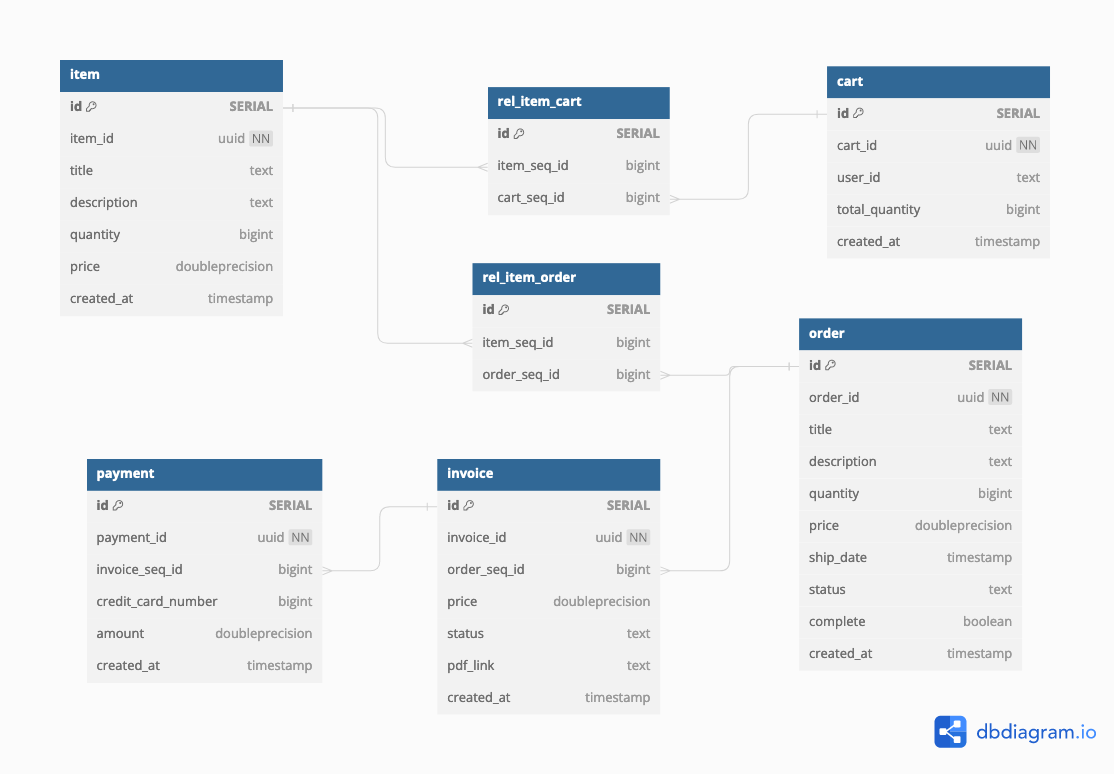
\includegraphics[width=\textwidth]{images/monolith_db_schema.png}
    \caption{Database schema displaying tables and relations of Monolithic example. \label{img:monolith_db_schema}}
\end{figure}



\subsection{Modulith}
This is example using Modular Monolith approach. The original Monolithic application was split into multiple smaller Monoliths called \textit{modules}. The scope of every module depends on the specificity of the project. In this case it nearly corresponds to module per database Entity, exception being shopping cart and items, which were merged into single module to demonstrate possibility to have modules with larger volume. Package schema and dependency is displayed on Diagram~\ref{img:modulith_package}.

Every module has the same internal structure as original Monolith plus exposes its API with interface (Diagram~\ref{img:modulith_module_package}). Modules encapsulate its own data storage and there shouldn't be any inter-modules table constraint set in database, although it is possible, it does not make sense from the perspective of logical separation and might be very confusing. It should be possible for every module to use different database and even different database technology. In case of the largest module containing shopping cart and items, there are foreign keys constraints preserved since it resides inside single module.

Module can use API of other modules, although this should be limited as much as possible to keep coupling low. Dependency on other modules is defined through usage of interfaces and the actual implementation can be either injects automatically using IoC approach or as in this case just defining top level module, which takes care of initializing individual modules and spinning up HTTP server.

Scaling Modulith once we identify the packages from which the bottleneck consists is very easy. Since every module is basically small Monolith, it can be separated into service and run independently. It just has to expose its API via network like gRPC or just simple HTTP api. This network expose step can be automatically generated if all objects in interface are serializable. Later client instances will be passed to all dependent modules and from point of view of other modules nothing changes, just now the underlying communication will not be inter-process communication, but network communication.

\begin{figure}
    \centering
    \includesvg[width=0.7\textwidth]{images/modulith_module_package.svg}
    \caption{Database schema displaying tables and relations. \label{img:modulith_module_package}}
\end{figure}

\begin{figure}
    \centering
    \includesvg[width=0.7\textwidth]{images/modulith_package.svg}
    \caption{Database schema displaying tables and relations. \label{img:modulith_package}}
\end{figure}

\subsubsection{Database}
Every module encapsulates its own tables completely independent of the rest. Table are the same as for Monolithic example on Diagram~\ref{img:monolith_db_schema}, but relation across modules were removed. The schema consist of four partitions with relations preserve within partition: first partition consist of invoice table, second of payment table, third order table with rel\_item\_order and last consist of tables item, cart and rel\_item\_cart.

% \begin{figure}
%     \centering
%     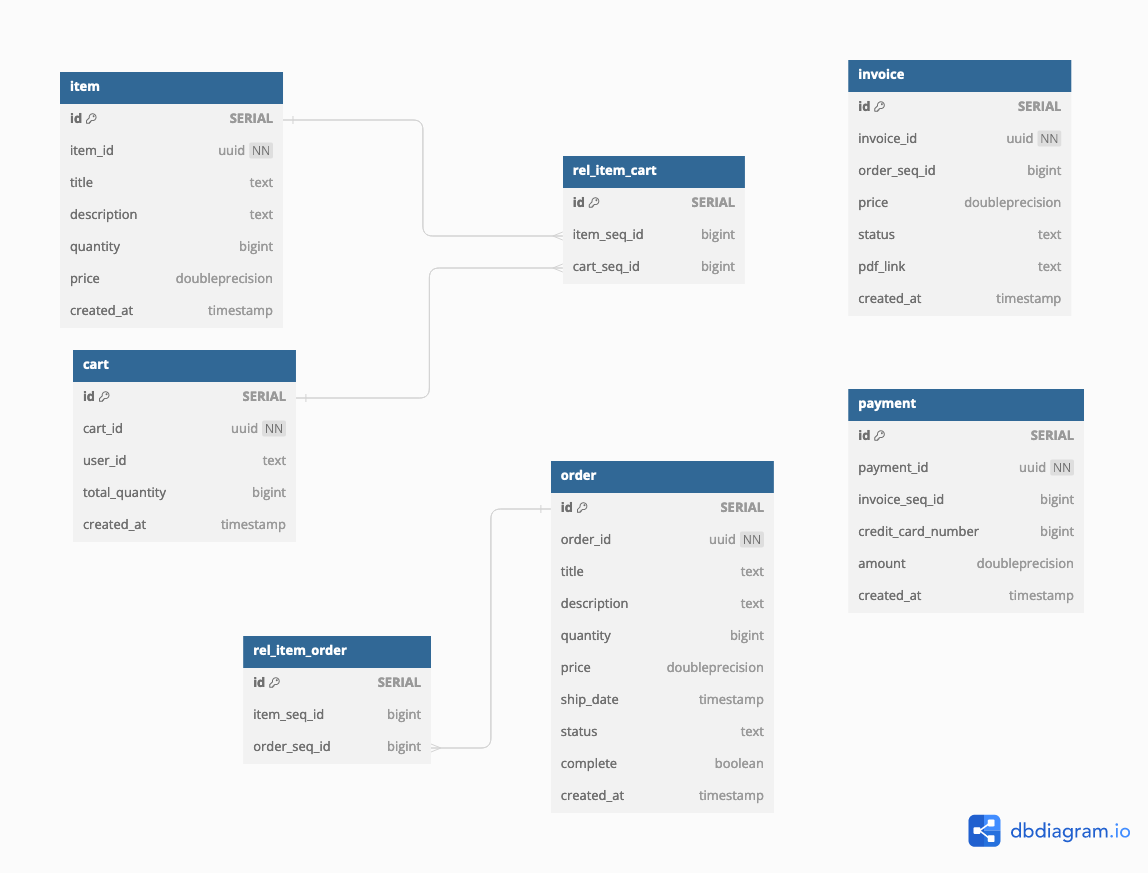
\includegraphics[width=\textwidth]{images/modulith_db_schema.png}
%     \caption{Database schema displaying tables and relations. \label{img:modulith_db_schema}}
% \end{figure}

\subsection{Microservices}
In this example the Modulith implementation was split into 5 micro-services: Item, Cart, Invoice, Order and Payment. Modulith originally contained 4 packages of which 1 was combined from logic around Shopping Cart and Items, so it was split into two for the volume to be more consistent across micro-services. The dependency graph between services is displayed on Diagram \ref{img:microservices_dependency}.

Every microservice is running HTTP server and exposing HTTP API for its internal API to be used by other modules and also public HTTP API to be used by clients. With microservices is common to use some kind of service discovery and let services communication with each other directly. In this example in order not to overcomplicate it was used nginx as load balancer, which acts as intermediary and forwards request to right services by path matching.

\begin{figure}
    \centering
    \includesvg[width=0.7\textwidth]{images/microservices_dependency.svg}
    \caption{Diagram displaying dependency between micro-services. \label{img:microservices_dependency}}
\end{figure}

\subsubsection{Database}
Every micro-service encapsulates its own data. Table are the same as for Monolithic example on Diagram~\ref{img:monolith_db_schema}, but constraints outside of micro-service scope were removed. The database partitions are the same as for Modulith, just Item table has been separate into its own service after splitting one package into two separate: cart and item.



\subsection{Benchmark methodology}
There are two types of scenarios, which will be measured to get inside into bottles of applications from both IO bound and CPU bound point of views. First one represents more even distributed requests, which should result in even application load (cpu intensive tasks vs IO tasks).
On the other hand the second should result in more cpu sensitive tasks and stress the system more.
Benchmark communicates with application via HTTP API and has defined following scenario displayed on Diagram \ref{img:benchmark_flow}.
Client load list of items (100) and adds one into his shopping cart. This repeats 10 times for first scenario and only once for second, after that he creates order, gets invoice information and pays for it.

\begin{figure}
    \centering
    \includesvg[width=0.7\textwidth]{images/benchmark_flow.svg}
    \caption{Benchmark flow diagram. \label{img:benchmark_flow}}
\end{figure}

All benchmarks results will originate from running 10 parallel tests and 100 iterations with following configuration.
\begin{itemize}
    \item Golang 1.21.3 - programming language used for applications
    \item PostgreSQL 14 - database
    \item Docker 24.0.5 - execution environment
    \item OpenTelemetry - monitoring from within application
    \item k6 - load testing tool
    \item Hardware - Macbook Air 13" with M2, 16 GB Ram, 6 CPU cores assigned to Docker
          % TODO this configuration might change for MicroServices -> we will see
    \item Every service instance has following reserved resources: 0.5~CPU and 50~MB of Ram
\end{itemize}mo

\subsection{Benchmark results (Alfa)}

In Table \ref{table:benchmark_baseline} are results of benchmark which will act as baseline. Both Monolith and Modulith were running in single instance with 0.5~CPU assigned and Microservices assigned 0.5~CPU per service. Even though both Monolith and Modulith are running as single process, there is already little overhead visible due to more complex internal structure and more database connection pools.

\begin{table}
    \begin{tabular}{ |p{3cm}||p{3cm}|p{1.5cm}|p{1.5cm}|p{1.5cm}|p{1.5cm}| }
        \hline
        \multicolumn{5}{|c|}{Benchmark results scenario 1}                   \\
        \hline
        Architecture  & Resources & rps        & avg     & p(90)   & p(95)   \\
        \hline
        Monolith      & 0.5\,CPU  & 6.8\,req/s & 1.43\,s & 1.2\,s  & 14.4\,s \\
        Modulith      & 0.5\,CPU  & 7.8\,req/s & 1.25\,s & 1.59\,s & 9.18\,s \\
        Microservices & 2.5\,CPU  & 6.9\,req/s & 1.43\,s & 1.1\,s  & 17.9\,s \\
        \hline
    \end{tabular}
    \caption{Table containing benchmark results comparing Monolith, Modulith and Microservices. Microservices and much more CPU reserved, since it consist of 5 services (every singe one has 0.5~CPU assigned).\label{table:benchmark_baseline}}
\end{table}

The biggest bottleneck of this benchmark is processing order due to CPU bound task. To scale Monolith we would have to run more instances, which for big systems is very resource demanding, and target of this theses is to focus on more modern architecture styles, so it will not be discussed further. On the other hand for modulith systems it is much easier due to its modular structure. The cpu bound task is contained inside invoice package, which can be moved into separate lightweight service and scaled as much as wanted.

In this example, invoice package was moved into separated service implementing HTTP server. HTTP client is than passed in main server to whoever module required the invoice interface. The same benchmark was run for one, two, four and eight instances of invoice service and results can be seen in Table~\ref{table:benchmark_modulith_instances} along with scaled Microservices example. There is no difference between Modulith and Modulith with single invoice service instance, but having the invoice service scaled to two instances, it has more then doubled the speed. Adding more instances scales linearly until the main bottleneck becomes IO bound task during payment. Microservices scale as well as Modulith, but having more overhead (more network inter-service communication) they are slightly slower.

\begin{table}
    \begin{tabular}{ |p{3cm}||p{3cm}|p{1.5cm}|p{1.5cm}|p{1.5cm}|p{1.5cm}| }
        \hline
        \multicolumn{5}{|c|}{Benchmark results scenario 1}                         \\
        \hline
        Architecture       & Resources & rps         & avg     & p(90)   & p(95)   \\
        \hline
        Modulith unified   & 0.5\,CPU  & 7.8\,req/s  & 1.25\,s & 1.59\,s & 9.1\,s  \\
        \rowcolor{Gray}
        Modulith + 1       & 1.0\,CPU  & 7.3\,req/s  & 1.35\,s & 1.0\,s  & 18.6\,s \\
        \rowcolor{Gray}
        Microservices      & 2.5\,CPU  & 6.9\,req/s  & 1.43\,s & 1.1\,s  & 17.9\,s \\
        Modulith + 2       & 1.5\,CPU  & 18.8\,req/s & 510\,ms & 605\,ms & 3.1\,s  \\
        Microservices  + 1 & 3.0\,CPU  & 21.4\,req/s & 441\,s  & 612\,ms & 3.9\,s  \\
        \rowcolor{Gray}
        Modulith + 4       & 2.5\,CPU  & 44.2\,req/s & 204\,ms & 521\,ms & 1.2\,s  \\
        \rowcolor{Gray}
        Microservices  + 3 & 4.0\,CPU  & 58.3\,req/s & 165\,ms & 513\,ms & 1.0\,s  \\
        Modulith + 8       & 4.5\,CPU  & 71.6\,req/s & 133\,ms & 512\,ms & 0.8\,s  \\
        Microservices  + 7 & 6.0\,CPU  & 66.4\,req/s & 142\,ms & 519\,ms & 0.9\,s  \\
        \hline
    \end{tabular}
    \caption{Table containing benchmark for Modulith and Microservices with module invoice moved into separate service running in multiple number of instances (indicated by number after plus sign, microservices has number by one lower, since by default there is already invoice service running).\label{table:benchmark_modulith_instances}}
\end{table}

% TODO for microservice benchmark look into CPU usage vs modulith cpu usage
% there seems to be big spike


% \subsection{Performance}

% latency
% throughput
% scalability
% 

% \subsection{Maintainability}
% Easy debugging | logging

% \subsection{Sustainability}
% transactions?

% \subsection{Testability}

% \subsection{Complexity}